% !TEX encoding = UTF-8 Unicode
\documentclass[12pt, A4,onecolumn]{article} %se puede poner twocolumn
\usepackage[normalem]{ulem} %tachar
\usepackage{cite}
\usepackage[utf8]{inputenc}
\usepackage{verbatim} %para comentarios 
%\usepackage[spanish]{babel}
\usepackage[hidelinks]{hyperref} %para que no salga en rojo
\usepackage{color} %para poder escribir con colores
\usepackage[margin=2.5cm]{geometry} %para modificar margenes
\usepackage{listings} %para insertar código
\usepackage[table,xcdraw]{xcolor} %para insertar tablas con color
\usepackage{amsmath} %para matrices
\usepackage{graphicx} %para insertar imagenes
\usepackage{float}
\usepackage{subcaption} % loads the caption package
\usepackage{multirow}
\definecolor{dkgreen}{rgb}{0,0.6,0}
\definecolor{gray}{rgb}{0.5,0.5,0.5}
\definecolor{mauve}{rgb}{0.58,0,0.82}
\graphicspath{ {Machintosh_HD/Utenti/admin/Scrivania} }


\title{\textbf{Machine Learning\\ 
\small{by Stanford University}\\
Week2
}}
\author{
Jose Vicente Yago Martínez
}%\date{28/3/2019}


\begin{document}
\maketitle

	
%\vfill
%\centering
%\textit{Lecturer:} \\
%AndrewNg


%\begin{figure}[H]
%	\centering
%	\includegraphics[width=0.2\textwidth]{logo-fium}
%\end{figure}	



\newpage
\tableofcontents
%\listoffigures

\newpage

% -----------------------------------------------------------------------------------%
% -----------------------------------------------------------------------------------%
%----------------MULTIVARIATE LINEAR REGRESSION--------------%
% -----------------------------------------------------------------------------------%
% -----------------------------------------------------------------------------------%
\section{Multivariate linear regression}

\subsection{Multiple features}

\begin{figure}[H]
	\centering
	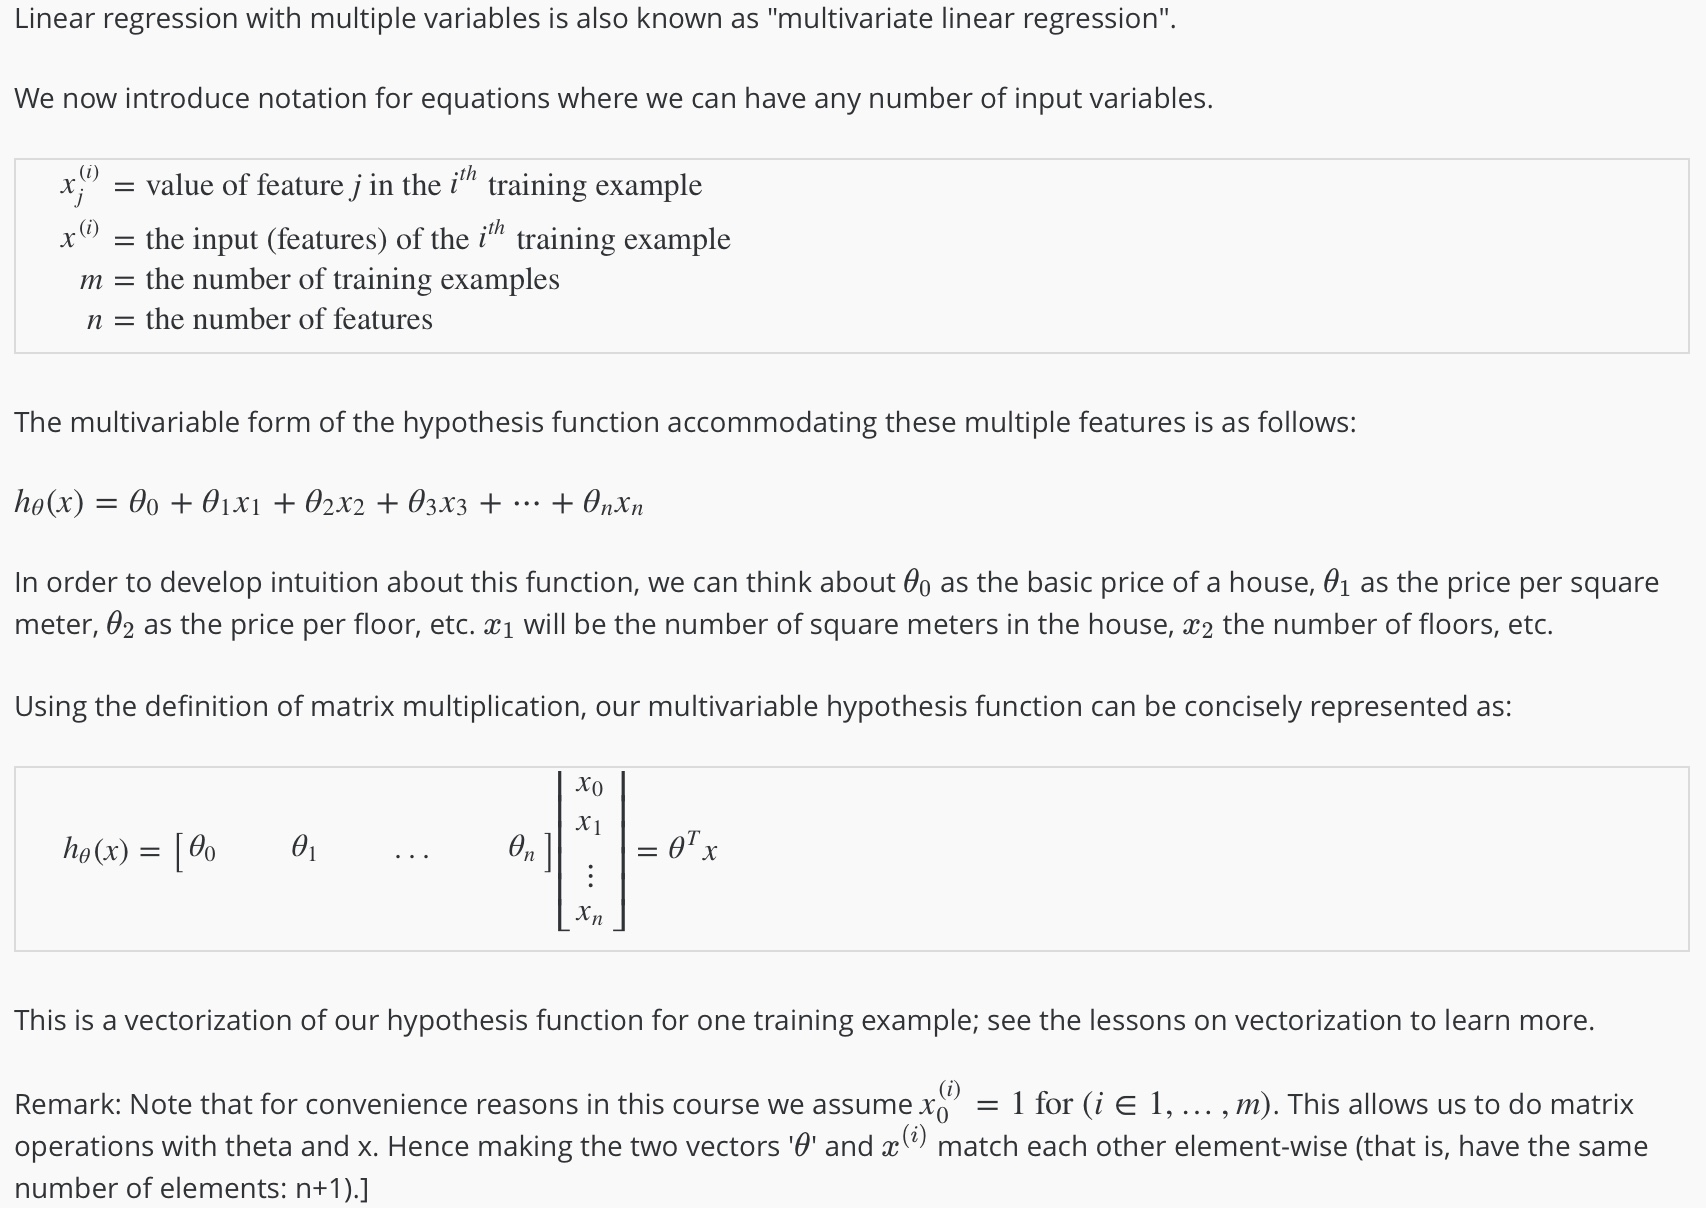
\includegraphics[width=1\textwidth]{./Imagenes/linreg1}
\end{figure}

\subsection{Gradient descent for multiple features}

\begin{figure}[H]
	\centering
	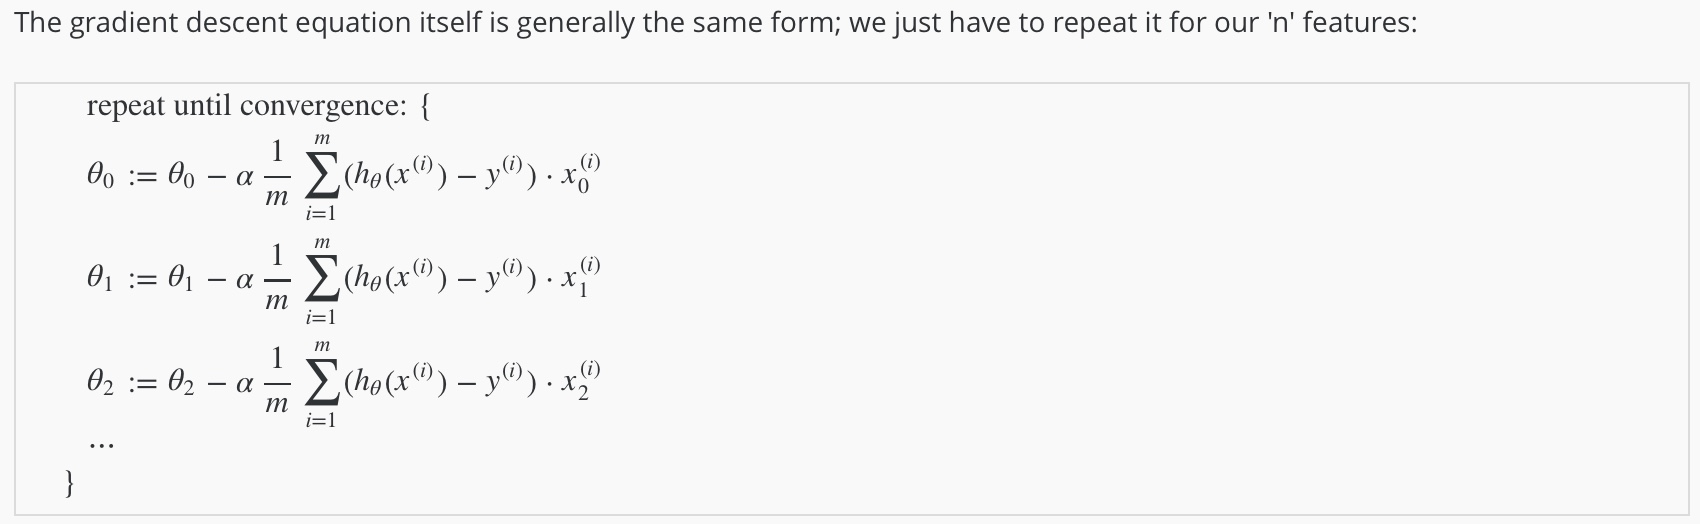
\includegraphics[width=1\textwidth]{./Imagenes/gradDes1}
\end{figure}

\begin{figure}[H]
	\centering
	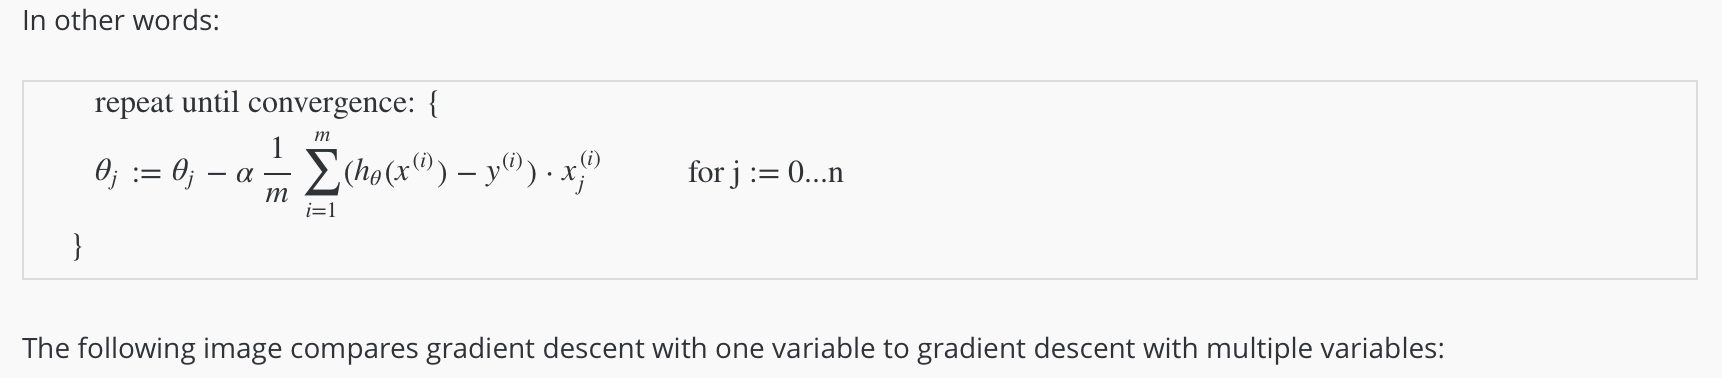
\includegraphics[width=1\textwidth]{./Imagenes/gradDes2}
\end{figure}

\begin{figure}[H]
	\centering
	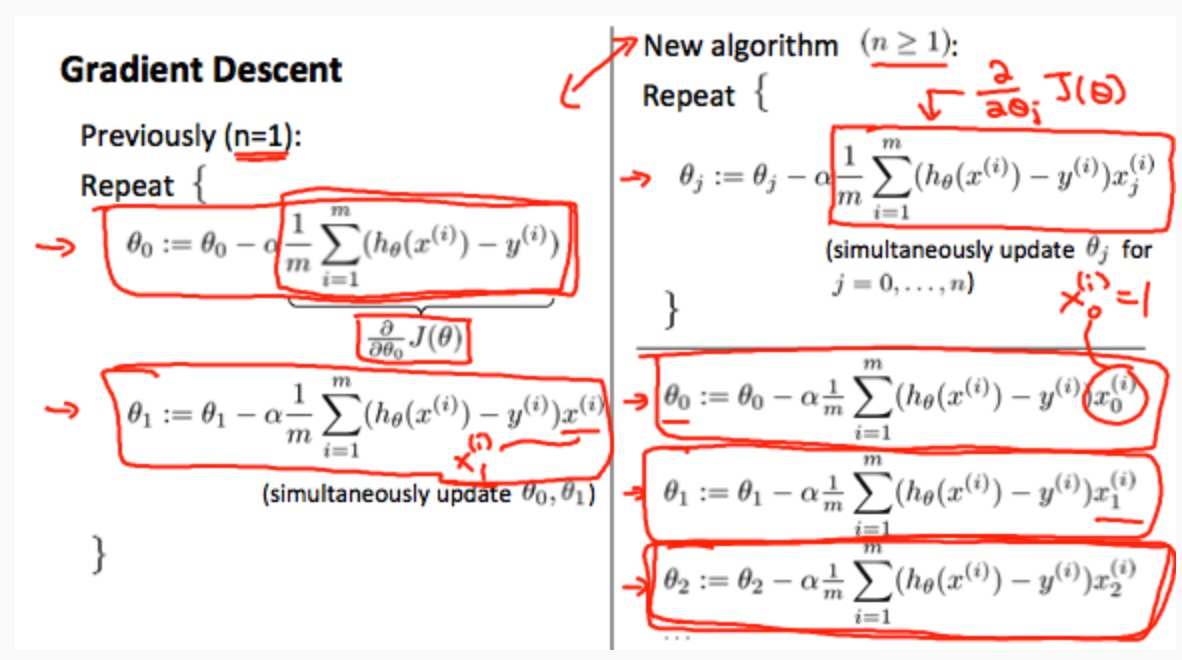
\includegraphics[width=1\textwidth]{./Imagenes/gradDes3}
\end{figure}


\subsection{Feature scaling}
\begin{figure}[H]
	\centering
	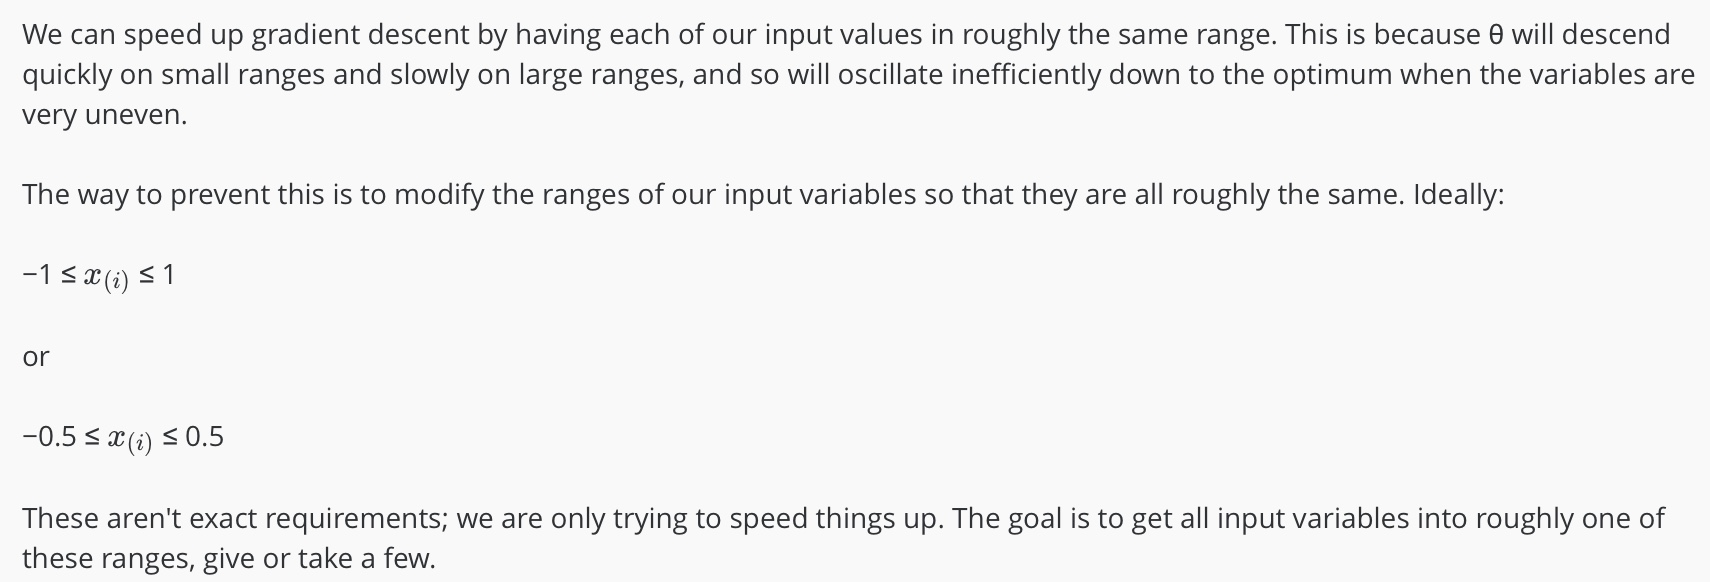
\includegraphics[width=1\textwidth]{./Imagenes/featScal1}
\end{figure}

\begin{figure}[H]
	\centering
	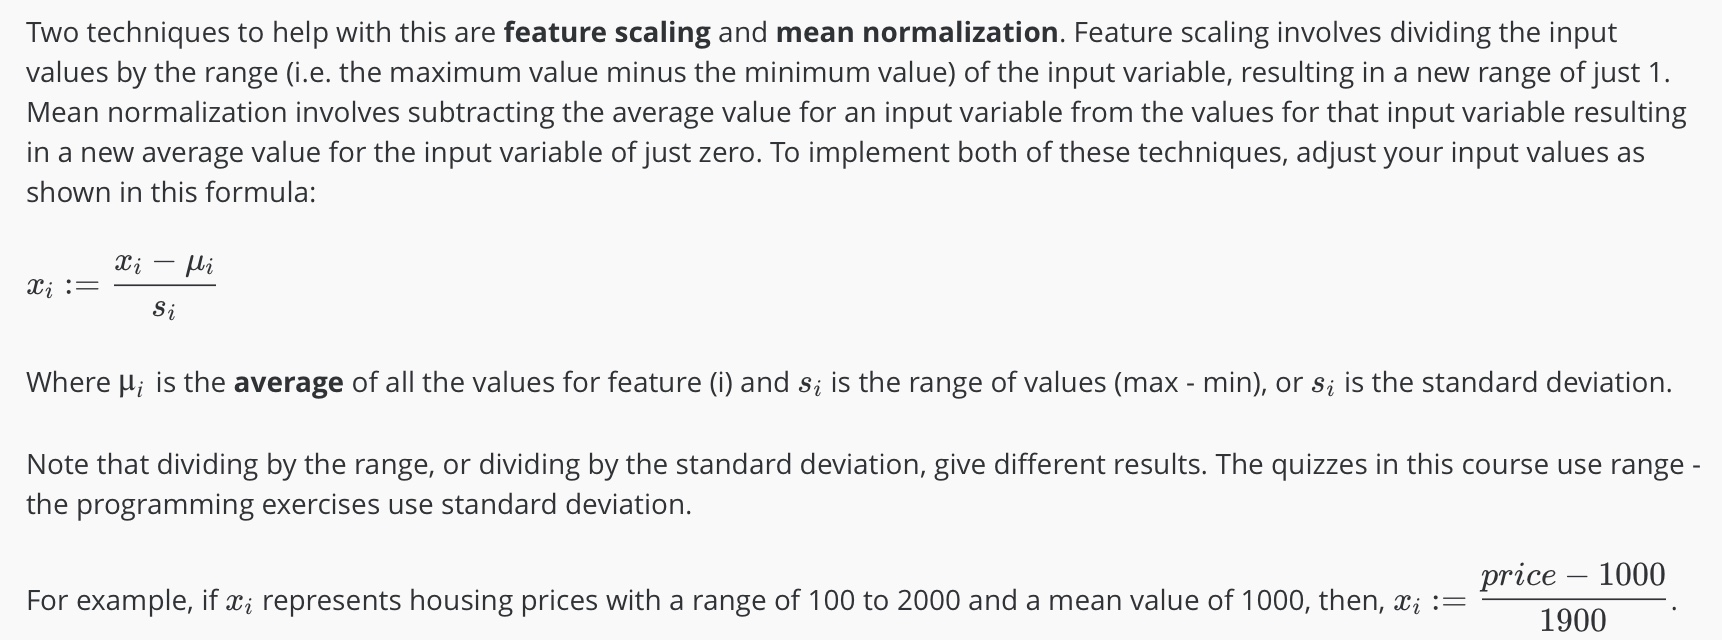
\includegraphics[width=1\textwidth]{./Imagenes/featScal2}
\end{figure}

\subsection{Learning rate}

\begin{figure}[H]
	\centering
	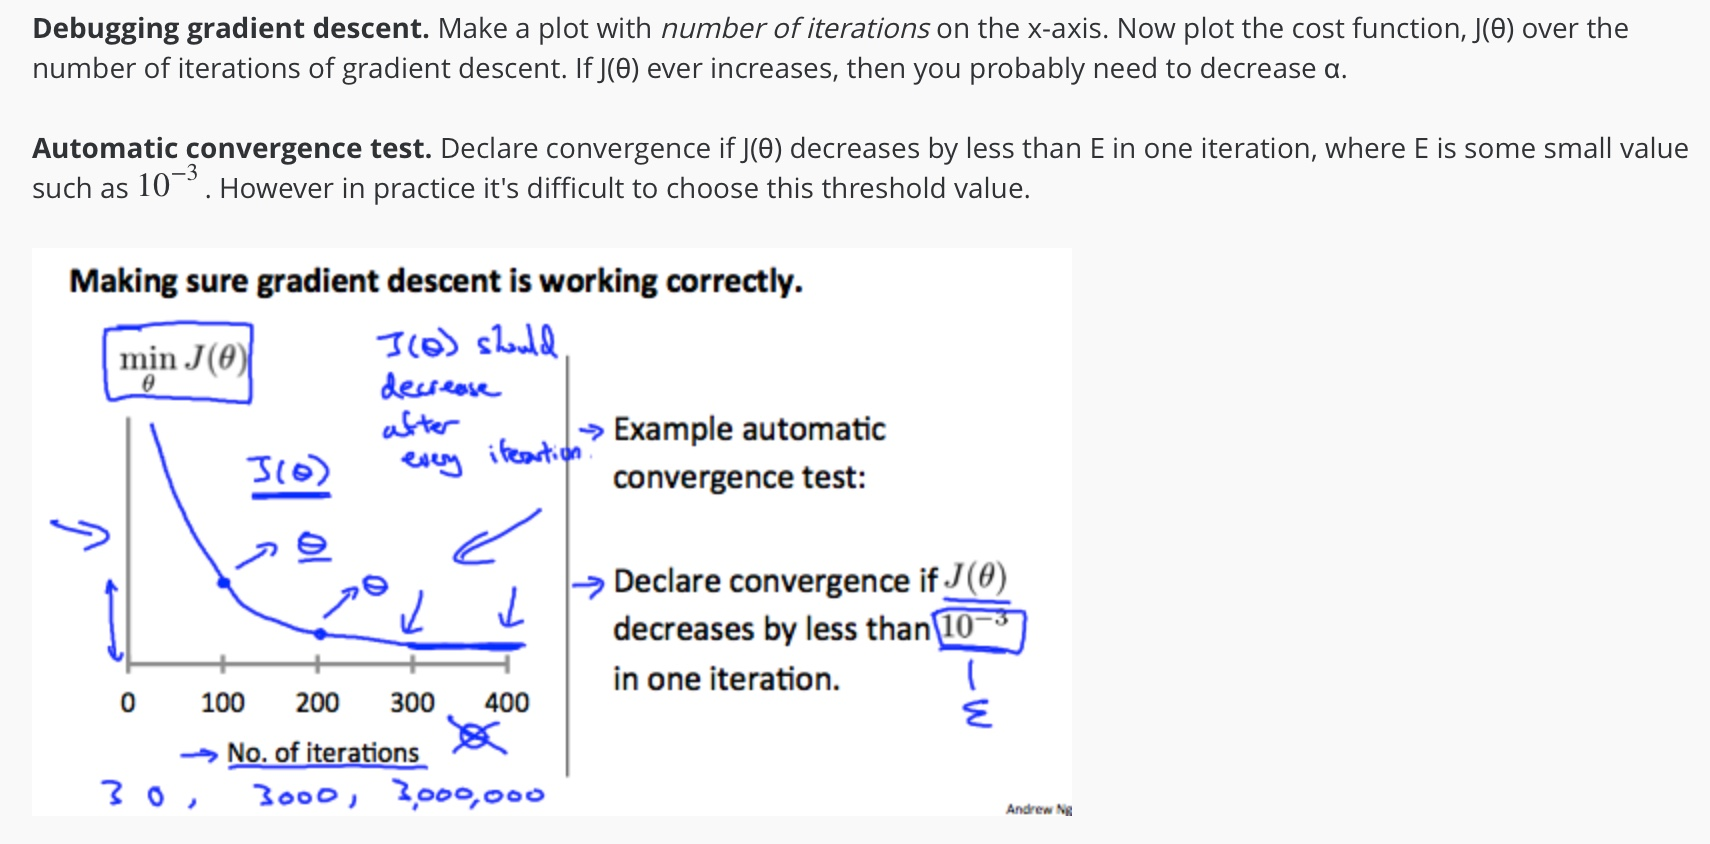
\includegraphics[width=0.8\textwidth]{./Imagenes/learnR1}
\end{figure}

\begin{figure}[H]
	\centering
	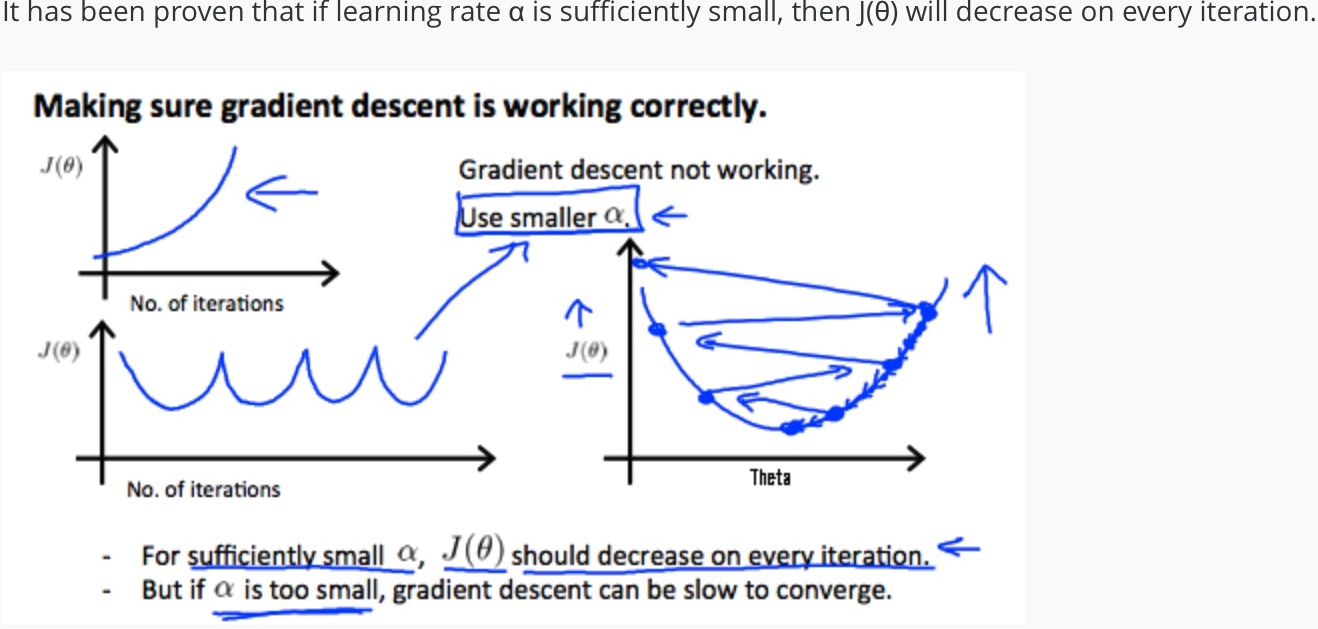
\includegraphics[width=0.8\textwidth]{./Imagenes/learnR2}
\end{figure}

\subsection{Features and polynomial regression}
\begin{figure}[H]
	\centering
	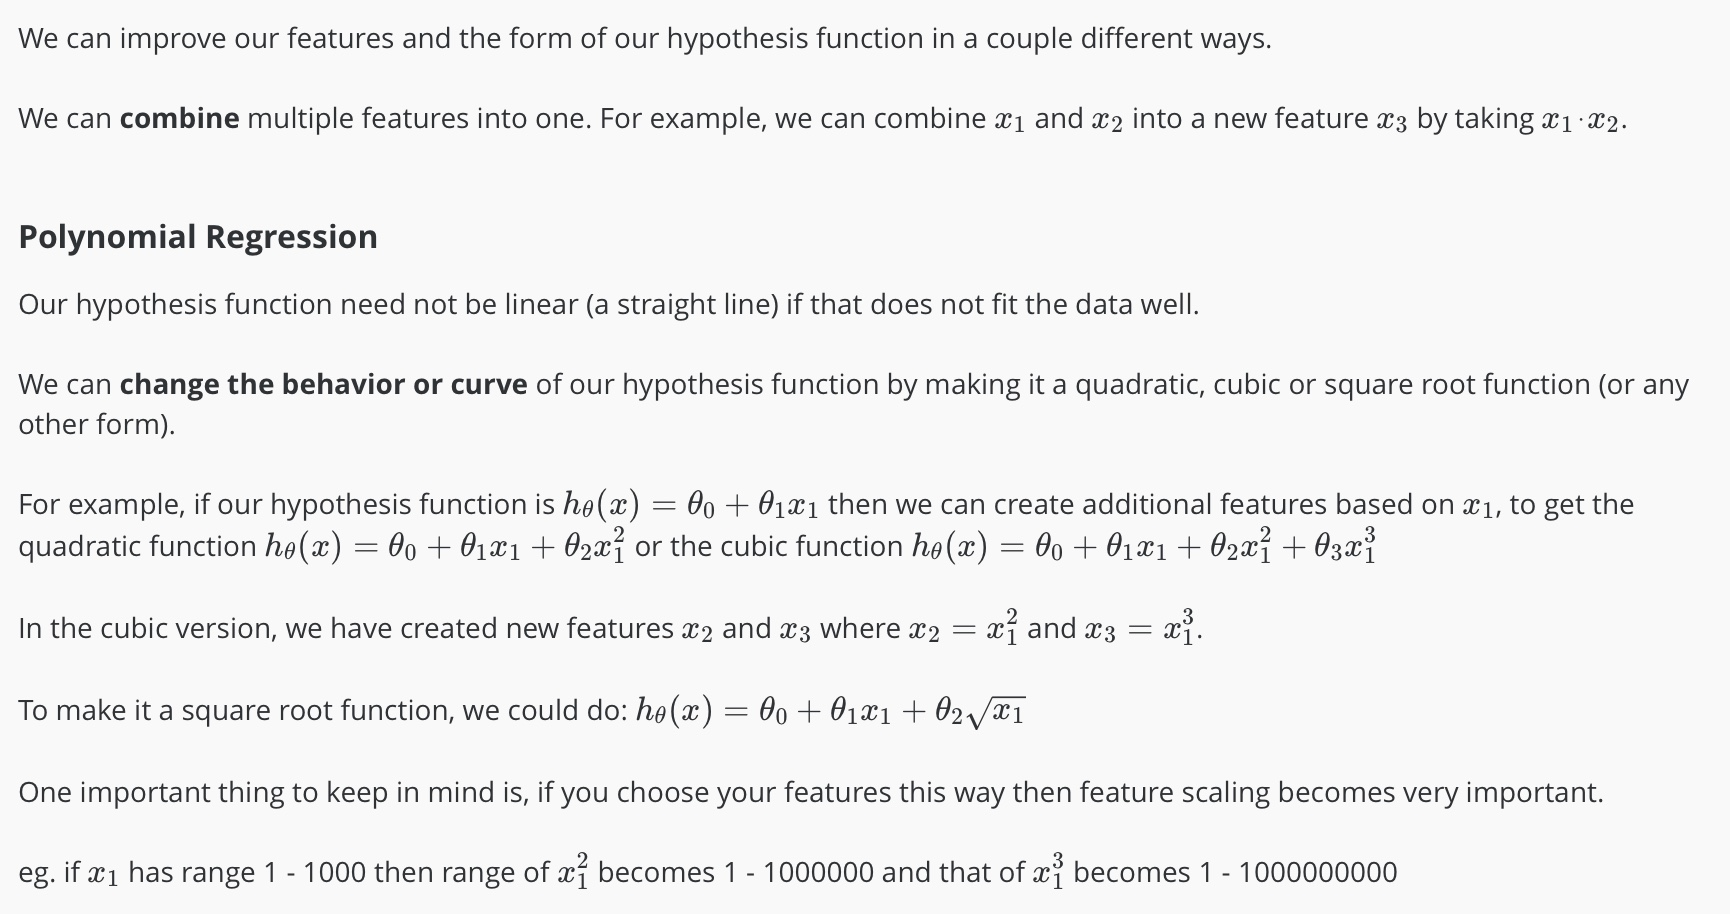
\includegraphics[width=1\textwidth]{./Imagenes/poly1}
\end{figure}

\begin{figure}[H]
	\centering
	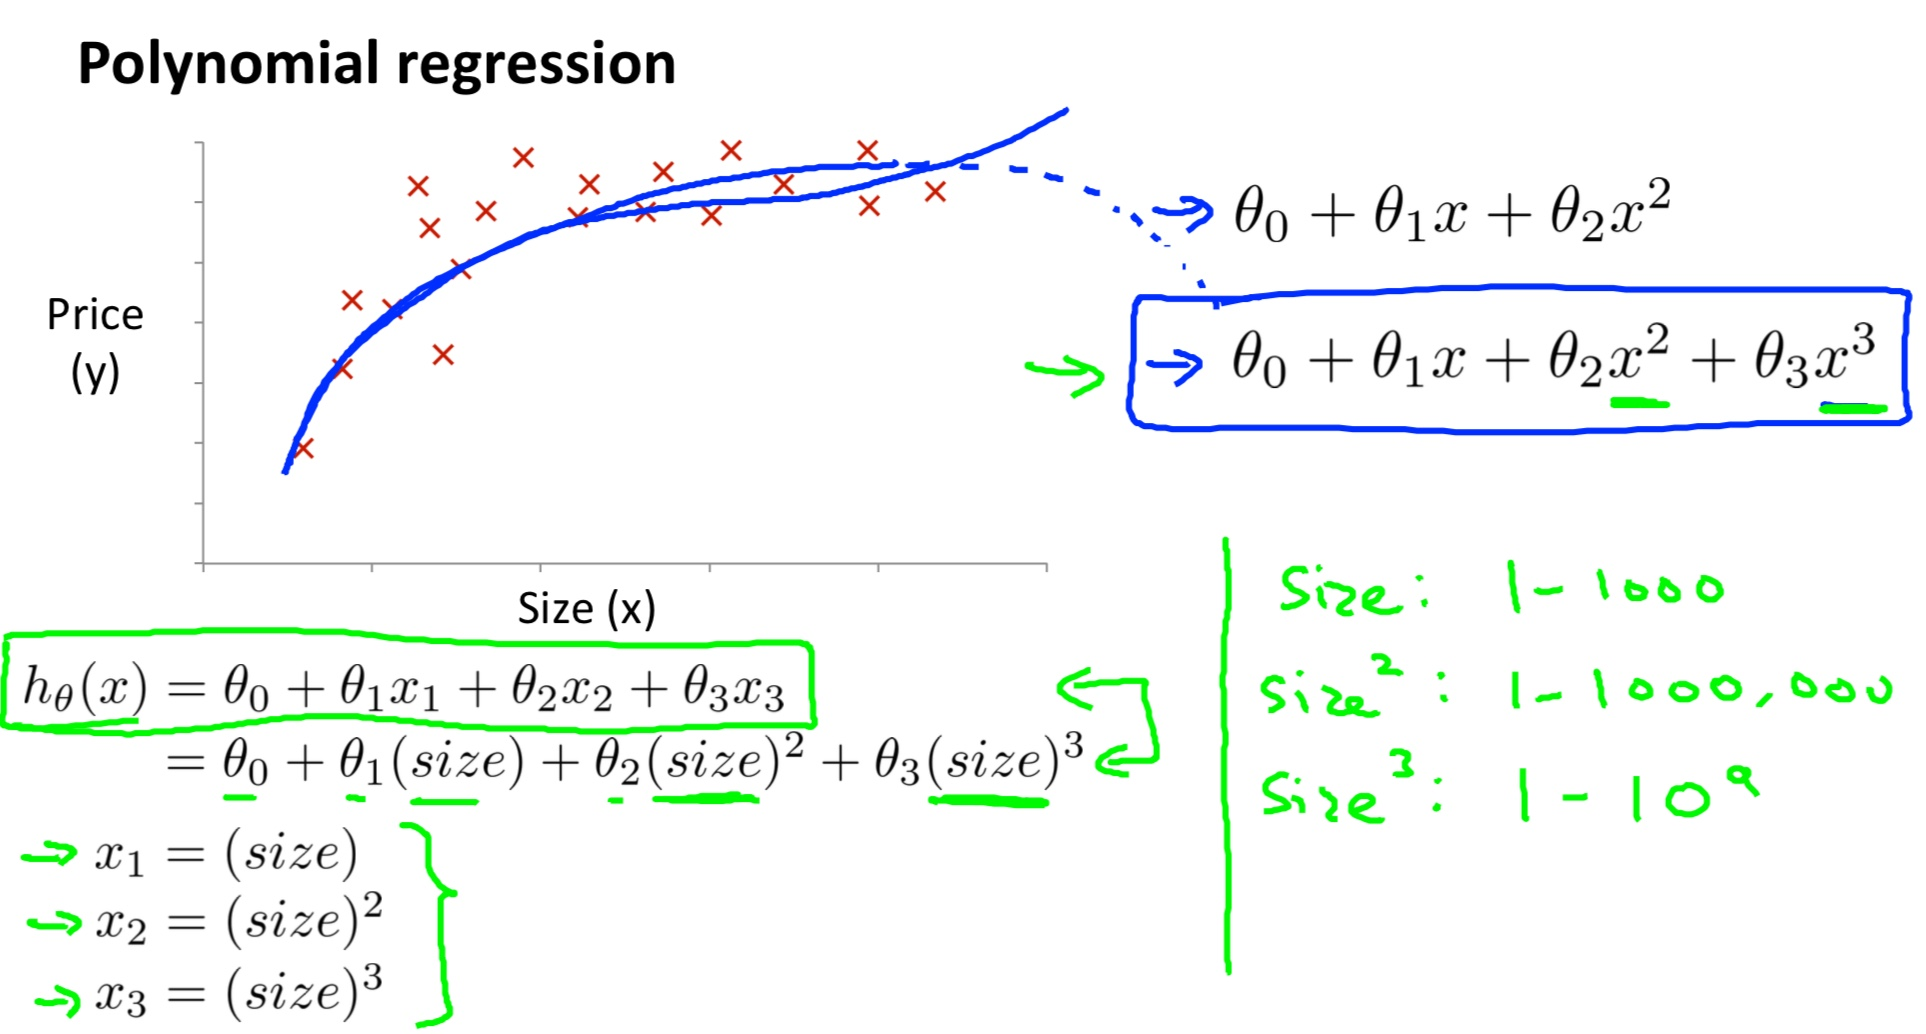
\includegraphics[width=1\textwidth]{./Imagenes/poly2}
\end{figure}

\begin{figure}[H]
	\centering
	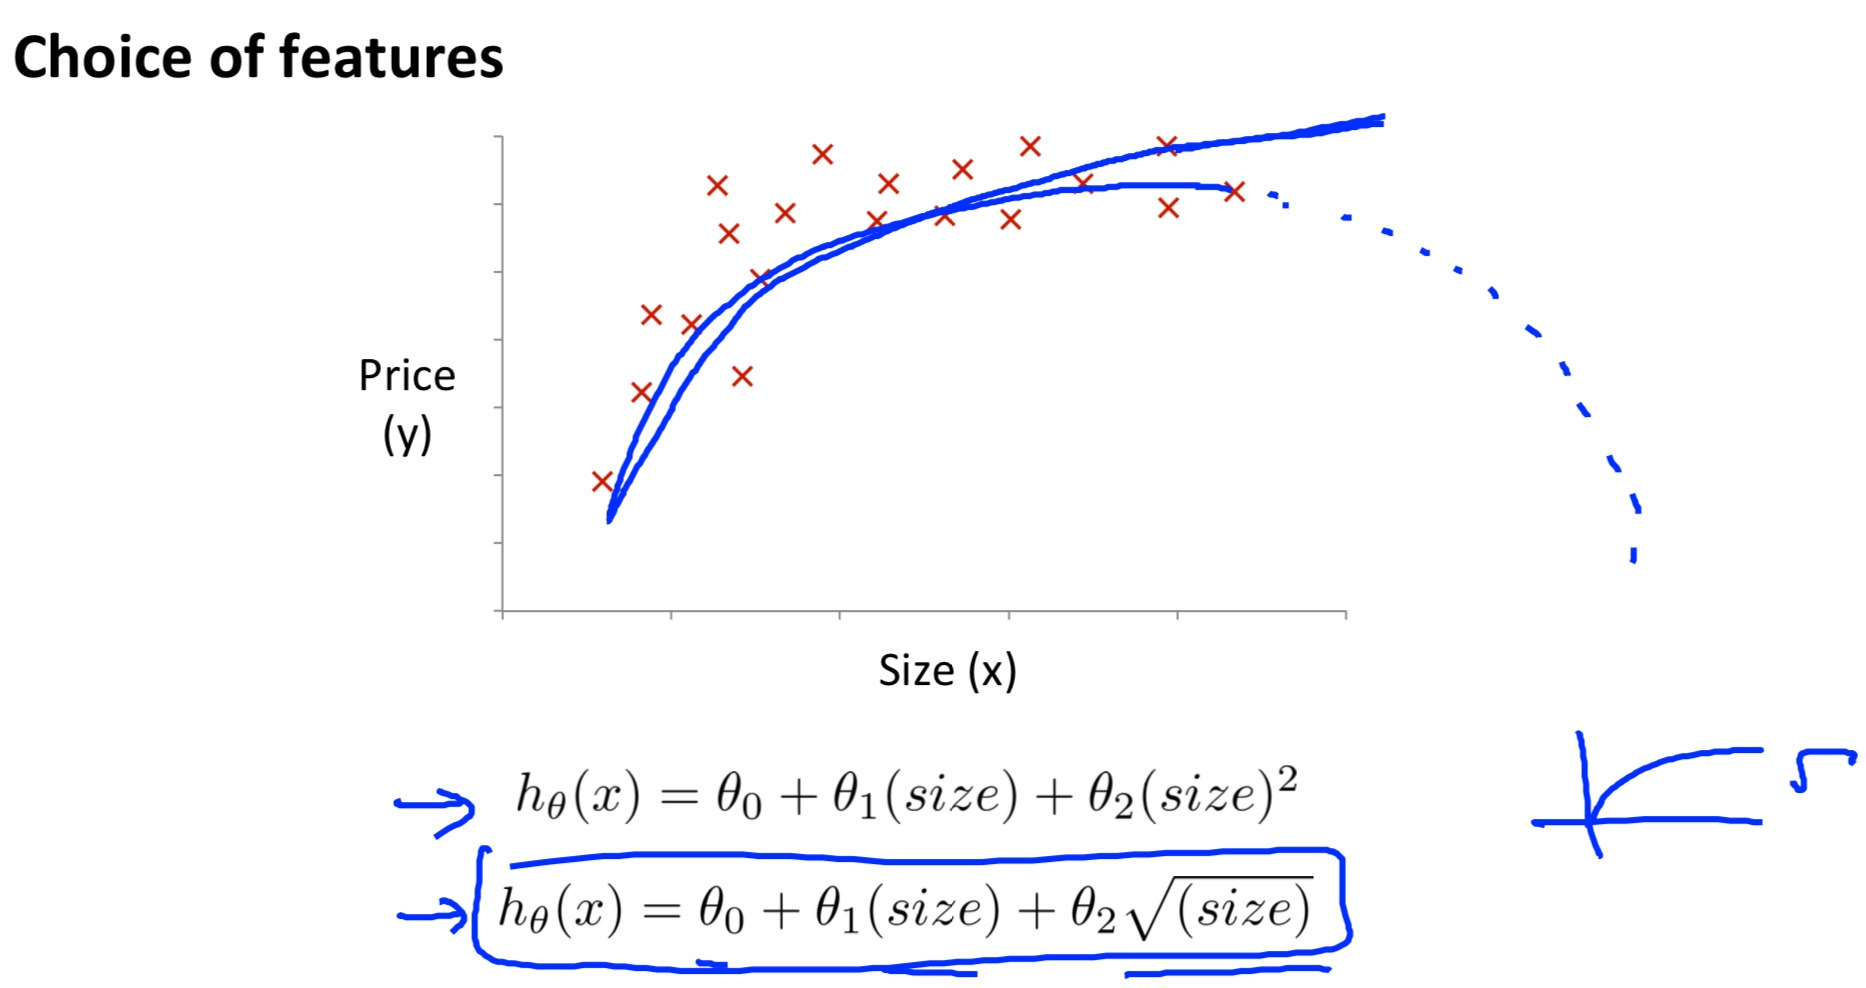
\includegraphics[width=1\textwidth]{./Imagenes/poly3}
\end{figure}

% -----------------------------------------------------------------------------------%
% -----------------------------------------------------------------------------------%
%----------COMPUTING PARAMETERS  ANALYTICALLY------------%
% -----------------------------------------------------------------------------------%
% -----------------------------------------------------------------------------------%
\section{Computing parameters analytically}
\subsection{Normal equation}
\begin{figure}[H]
	\centering
	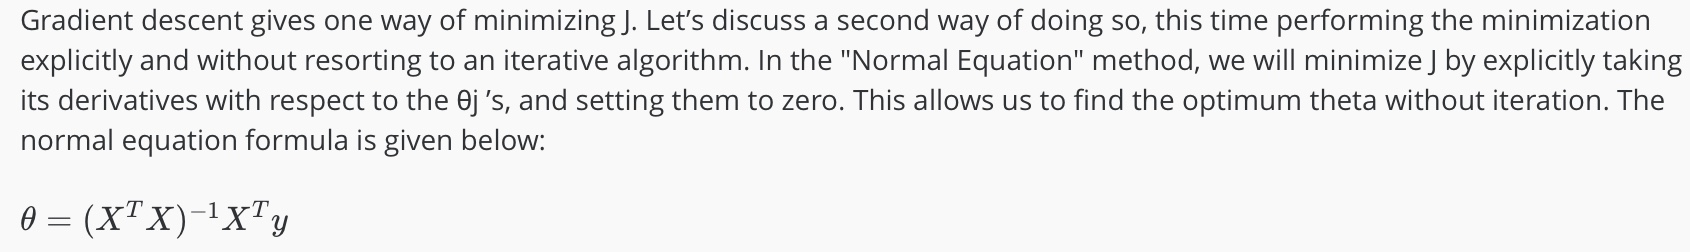
\includegraphics[width=0.85\textwidth]{./Imagenes/normalEq1}
\end{figure}
\begin{figure}[H]
	\centering
	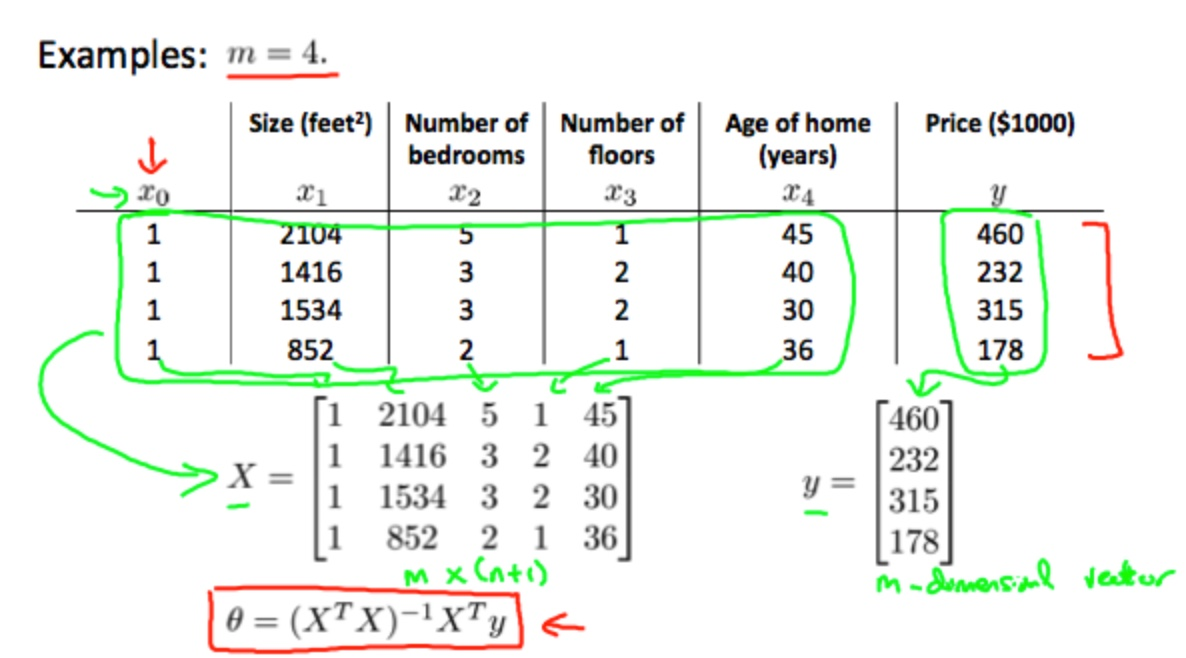
\includegraphics[width=0.9\textwidth]{./Imagenes/normalEq2}
\end{figure}
\begin{figure}[H]
	\centering
	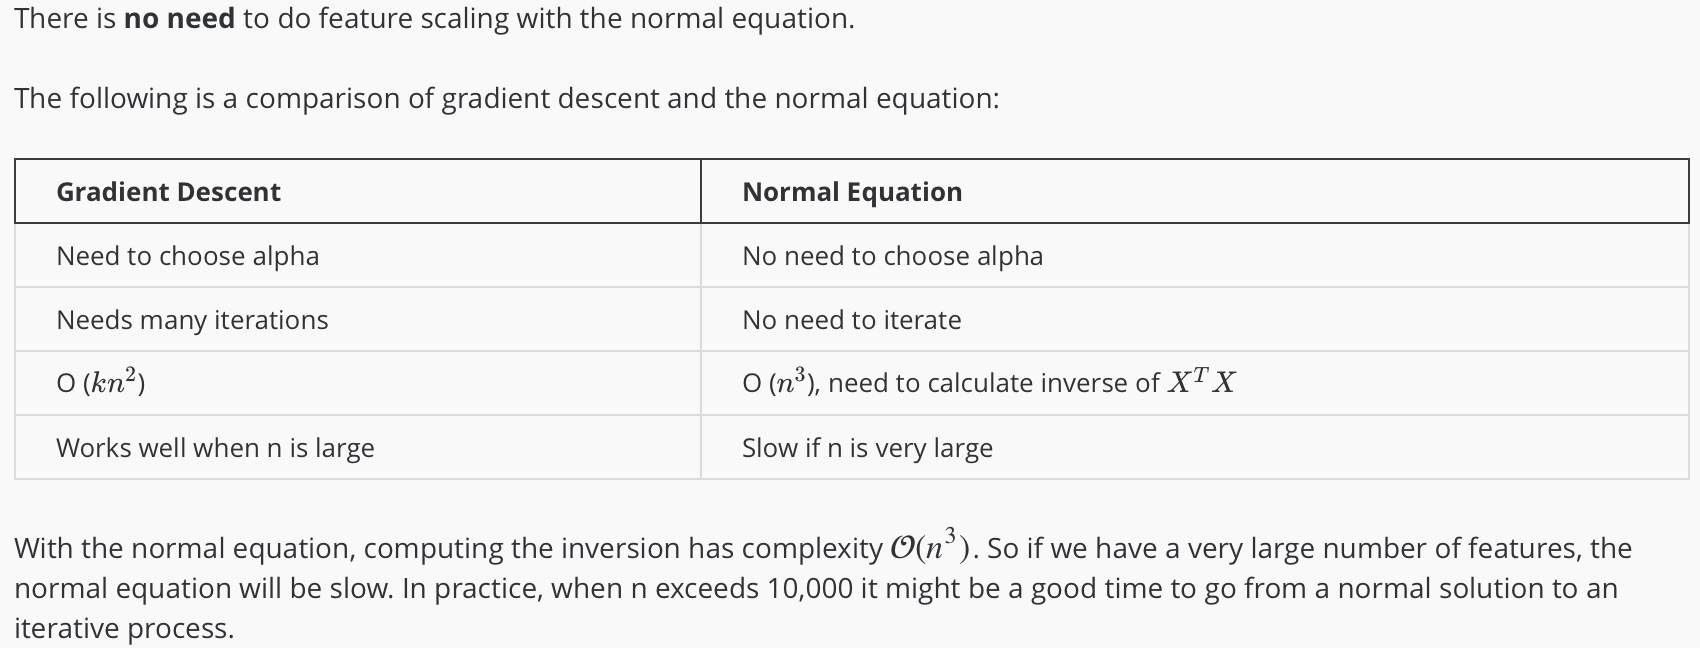
\includegraphics[width=1\textwidth]{./Imagenes/normalEq3}
\end{figure}

\subsubsection{Normal equation noninvertibility}
\begin{figure}[H]
	\centering
	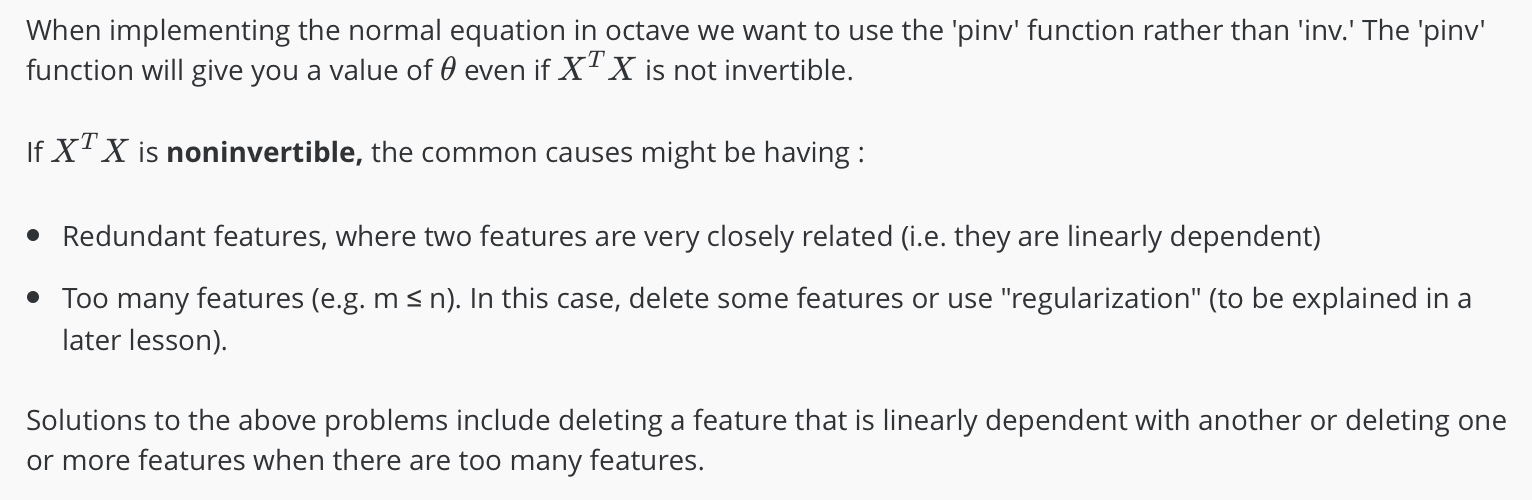
\includegraphics[width=1\textwidth]{./Imagenes/normalEq4}
\end{figure}

\end{document}
